\chapter{I princìpi di conservazione}

Nel capitolo precedente abbiamo incontrato l'\textbf{energia} e visto che il lavoro la trasferisce da un corpo all'altro e la fa cambiare forma. In questo capitolo ricaviamo alcune \textbf{leggi di conservazione}: affermazioni del tipo ``\emph{questa grandezza, per un sistema isolato, non cambia mai}''. Sono fra gli strumenti più potenti della fisica, perché permettono di mettere in relazione lo stato iniziale e quello finale di un sistema senza seguire in dettaglio tutto ciò che accade nel mezzo.

Ci occupiamo di due grandezze che, per un sistema isolato, restano costanti: l'\textbf{energia meccanica} e la \textbf{quantità di moto}.

\section[Conservazione dell'energia]{La conservazione dell'energia meccanica}

\subsection{L'energia meccanica}
Un tuffatore fermo sul trampolino possiede energia potenziale gravitazionale (rispetto all'acqua) ma non energia cinetica. Mentre si tuffa la quota diminuisce e la velocità aumenta: l'energia potenziale si trasforma in energia cinetica. Le due grandezze cambiano, ma conviene considerarne la \emph{somma}.

\begin{definizione}
La somma dell'energia cinetica e dell'energia potenziale gravitazionale di un corpo si chiama \textbf{energia meccanica}:
\[ \colorboxed{ocre}{ E_m = E_c + E_p. } \]
Si misura in joule.
\end{definizione}

\subsection{Il principio di conservazione dell'energia meccanica}
Consideriamo un sasso inizialmente fermo in un punto $A$ a quota $h_A$. La sua energia cinetica è nulla, quindi l'energia meccanica coincide con l'energia potenziale: $E_{mA} = m\,g\,h_A$.

Lasciamo cadere il sasso; dopo un po' si trova in un punto $B$ a quota $h_B < h_A$. L'energia potenziale è diminuita di $\Delta E_p = m\,g\,(h_A - h_B)$. In compenso il sasso ha acquistato velocità, quindi energia cinetica. Per il teorema dell'energia cinetica, l'aumento $\Delta E_c$ è uguale al lavoro dell'unica forza agente, il peso:
\[ \Delta E_c = L_{\text{peso}} = m\,g\,(h_A - h_B) = \Delta E_p^{\text{(diminuzione)}}. \]
L'energia cinetica aumenta esattamente di quanto diminuisce l'energia potenziale: la loro somma, l'energia meccanica, \textbf{non cambia}.

\begin{definizione}
\textbf{Principio di conservazione dell'energia meccanica.} Quando su un corpo agisce solo la forza-peso, la sua energia meccanica rimane costante:
\[ \colorboxed{ocre}{ E_{mA} = E_{mB}, \qquad \text{cioè}\quad E_{cA} + E_{pA} = E_{cB} + E_{pB}. } \]
\end{definizione}

Puoi pensare all'energia meccanica come a un gruzzolo di monete: puoi dividerlo come vuoi fra la ``tasca'' dell'energia cinetica e quella dell'energia potenziale, ma il totale non cambia. In particolare, quando il sasso arriva al suolo la sua energia potenziale è nulla e tutta l'energia meccanica è cinetica.

\begin{figure}[!htbp]
    \centering
    \begin{tikzpicture}[>=stealth]
        % traiettoria verticale
        \draw[->,thick] (0,-0.3) -- (0,4.6) node[left]{quota};
        \fill[ocre] (1.2,4) circle (2.5pt) node[right=3pt]{$A$};
        \fill[ocre] (1.2,0.3) circle (2.5pt) node[right=3pt]{$B$};
        \draw[gray,dashed] (0,4) -- (1.2,4);
        \draw[gray,dashed] (0,0.3) -- (1.2,0.3);
        \draw[<->] (-0.35,0.3) -- (-0.35,4) node[midway,fill=white,inner sep=1pt]{\footnotesize $h_A$};
        \draw[->,thick,ocre] (1.2,3.4) -- (1.2,2.4) node[midway,right]{\footnotesize $\vec v_B$};
        % barre di energia
        \foreach \x/\ec/\ep/\lab in {3.6/0/3/$A$, 6.0/3/0/$B$}{
            \draw (\x-0.35,0) rectangle (\x+0.35,3);
            \fill[blue!35] (\x-0.35,0) rectangle (\x+0.35,\ec);
            \fill[ocre!45] (\x-0.35,\ec) rectangle (\x+0.35,\ec+\ep);
            \node[below] at (\x,0) {\footnotesize \lab};
        }
        \node[blue!60!black,font=\footnotesize] at (6.0,-0.65) {$E_c$};
        \node[ocre,font=\footnotesize] at (3.6,-0.65) {$E_p$};
        \node[font=\footnotesize,align=center] at (4.8,3.5) {$E_m$ costante};
    \end{tikzpicture}
    \caption{Un sasso cade da $A$ a $B$: l'energia potenziale (arancione) si trasforma in energia cinetica (blu), ma la loro somma $E_m$ resta la stessa.}
    \label{fig:conservazione-sasso}
\end{figure}

\begin{remark}
Dal principio di conservazione si ricava subito la velocità di un corpo che cade da fermo da un'altezza $h$: tutta l'energia potenziale $m g h$ si trasforma in energia cinetica $\tfrac12 m v^2$, quindi
\[ \frac12\,m\,v^2 = m\,g\,h \;\Longrightarrow\; v = \sqrt{2\,g\,h}. \]
È la stessa formula ottenuta in cinematica con la ``formula senza il tempo'', e \textbf{non dipende dalla massa}.
\end{remark}

\begin{testexample}[\thetcbcounter \, Un tuffo dal trampolino]
Un tuffatore si lascia cadere da fermo da un trampolino alto \SI{5,0}{\metre} sopra l'acqua. Con che velocità entra in acqua (attrito dell'aria trascurabile)?

L'energia meccanica si conserva. In cima è tutta potenziale, all'ingresso in acqua tutta cinetica:
\[ \frac12\,m\,v^2 = m\,g\,h \;\Longrightarrow\; v = \sqrt{2\,g\,h} = \sqrt{2 \cdot 9{,}81 \cdot 5{,}0} \approx \SI{9,9}{\metre\per\second}. \]
\end{testexample}

\subsection{L'energia meccanica nei moti curvilinei}
Il principio vale \emph{qualunque sia il percorso} seguito dal corpo, non solo nella caduta verticale. Consideriamo una biglia che scende lungo una rampa curva liscia (figura~\ref{fig:pendolo-energia}): mentre scende, la forza-peso compie lavoro. Ma il peso è una forza \textbf{conservativa}: il suo lavoro non dipende dalla forma della traiettoria, ma \emph{solo dalla differenza di quota}. Quando la biglia arriva in fondo, la sua energia cinetica è di nuovo $m\,g\,(h_A - h_B)$, esattamente come nella caduta libera.

Lo stesso accade per un \textbf{pendolo}: lasciato andare da un punto $A$, arriva nel punto più basso con velocità massima (tutta l'energia è cinetica), poi risale dall'altra parte fino a raggiungere la \emph{stessa quota} di partenza, dove si ferma un istante (tutta l'energia è di nuovo potenziale).

\begin{figure}[!htbp]
    \centering
    \begin{tikzpicture}[>=stealth,scale=1]
        \def\R{2.9}
        % soffitto (tratteggio verso l'alto, dal lato del materiale fisso)
        \draw[thick] (-0.5,0) -- (0.5,0);
        \foreach \x in {-0.4,-0.2,0,0.2,0.4}{\draw (\x,0) -- (\x-0.16,0.16);}
        \fill (0,0) circle (1.3pt);
        % la traiettoria e' l'arco 215-325 gradi: passa per A (215), O (270), B (325)
        \coordinate (A) at (215:\R);
        \coordinate (O) at (270:\R);
        \coordinate (B) at (325:\R);
        \draw[gray!55,very thick] (215:\R) arc (215:325:\R);
        \draw[thin,gray] (0,0) -- (A);
        \draw[thin,gray,dashed] (0,0) -- (B);
        \fill[ocre] (A) circle (3pt) node[left=3pt]{\footnotesize $A$};
        \fill[ocre] (O) circle (3pt);
        \fill[ocre] (B) circle (3pt) node[right=3pt]{\footnotesize $B$};
        \node[font=\footnotesize,align=center,above left=1pt] at (A) {$E_p$ max\\$E_c=0$};
        \node[font=\footnotesize,align=center,above right=1pt] at (B) {$E_p$ max\\$E_c=0$};
        \node[font=\footnotesize,align=center,below=2pt] at (O) {punto più basso\\$E_c$ max, $E_p=0$};
        % dislivello h fra il livello di A/B e il punto piu' basso
        \draw[gray,dashed] (A) -- ($(A -| B)+(0.7,0)$);
        \draw[gray,dashed] (O) -- ($(O -| B)+(0.7,0)$);
        \draw[<->] ($(A -| B)+(0.5,0)$) -- ($(O -| B)+(0.5,0)$) node[midway,right]{\footnotesize $h$};
    \end{tikzpicture}
    \caption{Pendolo (attrito trascurabile): l'energia passa da potenziale a cinetica e di nuovo a potenziale. Il corpo risale sempre fino alla quota di partenza.}
    \label{fig:pendolo-energia}
\end{figure}

\begin{testexample}[\thetcbcounter \, La palla da demolizione]
Una palla da demolizione di massa \SI{200}{\kilo\gram} è legata a un cavo lungo $L = \SI{15}{\metre}$; viene sollevata di un angolo $\alpha = 45^\circ$ rispetto alla verticale e lasciata andare. Con che velocità arriva nel punto più basso, dove colpisce l'edificio?

Prima calcoliamo di quanto si abbassa. La distanza verticale fra il punto di sospensione e la palla, quando il cavo è inclinato di $\alpha$, è $L\cos\alpha$; nel punto più basso è $L$. Quindi la palla si abbassa di
\[ h = L - L\cos\alpha = 15 \cdot (1 - \cos 45^\circ) \approx 15 \cdot 0{,}293 \approx \SI{4,4}{\metre}. \]
Per la conservazione dell'energia meccanica, la velocità nel punto più basso è
\[ v = \sqrt{2\,g\,h} = \sqrt{2 \cdot 9{,}81 \cdot 4{,}4} \approx \SI{9,3}{\metre\per\second}, \]
indipendente dalla massa della palla.
\end{testexample}

\subsection{L'energia meccanica nei sistemi con corpi elastici}
Un corpo elastico (una molla) può immagazzinare energia meccanica sotto forma di \textbf{energia potenziale elastica} $E_e$, come abbiamo visto nel capitolo precedente. In un sistema in cui compare una molla, l'energia meccanica totale è
\[ E_m = E_c + E_p + E_e. \]

Nella figura~\ref{fig:carrello-molla} un carrello di massa $m$ si muove a velocità $v$ su un piano orizzontale liscio, con energia cinetica $\tfrac12 m v^2$. Quando urta una molla la comprime, compiendo lavoro; alla fine il carrello si ferma e la sua energia cinetica è nulla. Il lavoro di compressione è uguale all'energia potenziale elastica accumulata:
\[ \frac12\,m\,v^2 = \frac12\,k\,s^2. \]
L'energia meccanica del sistema è rimasta costante: si è solo trasferita dal carrello alla molla.

\begin{figure}[!htbp]
    \centering
    \begin{tikzpicture}[>=stealth]
        \def\rw{0.14}
        % istante 1
        \begin{scope}
            \draw[thick] (0,0) -- (5.2,0);
            \draw[fill=gray!20] (0.9,{2*\rw}) rectangle (2.1,{2*\rw+0.55});
            \draw[fill=gray!35] (1.2,\rw) circle (\rw); \draw[fill=gray!35] (1.8,\rw) circle (\rw);
            \draw[decorate,decoration={coil,segment length=4pt,amplitude=3.5pt}] (4.9,{2*\rw+0.27}) -- (2.9,{2*\rw+0.27});
            \draw[thick] (4.9,0) -- (4.9,{2*\rw+0.55});
            \draw[->,very thick,blue!60!black] (2.2,{2*\rw+0.75}) -- (3.0,{2*\rw+0.75}) node[right]{$\vec v$};
            \node[font=\footnotesize] at (2.6,-0.4) {$E_c = \tfrac12 m v^2$};
        \end{scope}
        % istante 2
        \begin{scope}[shift={(6.6,0)}]
            \draw[thick] (0,0) -- (5.2,0);
            \draw[fill=gray!20] (2.5,{2*\rw}) rectangle (3.7,{2*\rw+0.55});
            \draw[fill=gray!35] (2.8,\rw) circle (\rw); \draw[fill=gray!35] (3.4,\rw) circle (\rw);
            \draw[decorate,decoration={coil,segment length=2.6pt,amplitude=3.5pt}] (4.9,{2*\rw+0.27}) -- (3.75,{2*\rw+0.27});
            \draw[thick] (4.9,0) -- (4.9,{2*\rw+0.55});
            \draw[<->] (3.75,{2*\rw+0.9}) -- (4.9,{2*\rw+0.9}) node[midway,fill=white,inner sep=1pt]{\footnotesize $s$};
            \node[font=\footnotesize] at (2.6,-0.4) {$E_e = \tfrac12 k s^2$};
        \end{scope}
    \end{tikzpicture}
    \caption{Il carrello in moto cede la sua energia cinetica alla molla, che la immagazzina come energia potenziale elastica. L'energia meccanica del sistema resta costante.}
    \label{fig:carrello-molla}
\end{figure}

\begin{esercizio}
Un sasso è lasciato cadere da fermo da un ponte alto \SI{20}{\metre}. Usando la conservazione dell'energia meccanica, calcola la velocità con cui arriva all'acqua (attrito trascurabile).\\
\risp{$v = \sqrt{2\,g\,h} = \sqrt{2 \cdot 9{,}81 \cdot 20} \approx \SI{19,8}{\metre\per\second}$}
\end{esercizio}

\begin{esercizio}
Una biglia di massa \SI{50}{\gram} scende da ferma lungo una guida curva liscia partendo da un'altezza di \SI{1,2}{\metre}. Qual è la sua energia meccanica? Con che velocità arriva in fondo?\\
\risp{$E_m = m g h \approx \SI{0,59}{\joule}$; \; $v = \sqrt{2 g h} \approx \SI{4,9}{\metre\per\second}$}
\end{esercizio}

\begin{esercizio}
Un pendolo è lasciato andare da fermo da una posizione in cui è più alto di \SI{15}{\centi\metre} rispetto al punto più basso. Che velocità ha nel punto più basso?\\
\risp{$v = \sqrt{2 g h} = \sqrt{2 \cdot 9{,}81 \cdot 0{,}15} \approx \SI{1,7}{\metre\per\second}$}
\end{esercizio}

\begin{esercizio}
Una ragazza su uno skateboard (massa complessiva \SI{55}{\kilo\gram}) è ferma in cima a una rampa alta \SI{2,4}{\metre} rispetto alla pista. Qual è la sua energia meccanica nel punto più alto? A che velocità arriverebbe in fondo, se non ci fossero attriti?\\
\risp{$E_m = m g h \approx \SI{1,3e3}{\joule}$; \; $v = \sqrt{2 g h} \approx \SI{6,9}{\metre\per\second} \approx \SI{25}{\kilo\metre\per\hour}$}
\end{esercizio}

\begin{esercizio}
Una molla di costante elastica \SI{2,0}{\kilo\newton\per\metre} viene compressa di \SI{5,0}{\centi\metre}. Lasciata libera, lancia una biglia di massa \SI{20}{\gram}. Quale velocità acquista la biglia (attriti trascurabili)?\\
\risp{$\tfrac12 k s^2 = \tfrac12 m v^2 \Rightarrow v = s\sqrt{k/m} = 0{,}050\sqrt{2000/0{,}020} \approx \SI{16}{\metre\per\second}$}
\end{esercizio}

\begin{esercizio}
Un corpo di massa \SI{2,0}{\kilo\gram} viene lanciato verticalmente verso l'alto con velocità \SI{12}{\metre\per\second}. Usando la conservazione dell'energia, calcola l'altezza massima che raggiunge.\\
\risp{$\tfrac12 m v^2 = m g h \Rightarrow h = v^2/(2g) = 144/19{,}62 \approx \SI{7,3}{\metre}$}
\end{esercizio}

\section[Energia meccanica e attrito]{Quando l'energia meccanica non si conserva}

\subsection{L'attrito trasforma l'energia meccanica in calore}
Una pallina che oscilla su un profilo curvilineo \emph{reale} non risale mai fino alla quota di partenza: a ogni oscillazione arriva un po' più in basso, finché si ferma. Mentre si muove, l'attrito con la pista le fa perdere energia meccanica. E si osserva che, contemporaneamente, la pallina e la pista si \textbf{scaldano}.

\begin{definizione}
Le forze di attrito fanno \textbf{diminuire} l'energia meccanica di un corpo e producono un aumento di temperatura dei corpi a contatto. L'energia meccanica perduta si trasforma in \textbf{energia termica} (calore).
\end{definizione}

\subsection{Lavoro dell'attrito ed energia meccanica}
Sappiamo dal teorema dell'energia cinetica che la variazione di energia cinetica è uguale al lavoro delle forze agenti. Lo stesso vale per l'energia meccanica.

\begin{definizione}
Se un corpo soggetto al peso e all'\textbf{attrito} si muove da un punto $A$ a un punto $B$ lungo un percorso qualsiasi, la sua energia meccanica varia di una quantità pari al lavoro $L_a$ compiuto dalla forza di attrito:
\[ \colorboxed{ocre}{ E_{mB} - E_{mA} = L_a. } \]
Poiché l'attrito si oppone sempre al moto, $L_a$ è \textbf{negativo}: l'energia meccanica diminuisce.
\end{definizione}

Su un tratto rettilineo lungo $d$, con forza di attrito di modulo $F_a$, il lavoro dell'attrito vale $L_a = -F_a\,d$.

\begin{remark}
Non tutte le forze diverse dal peso ``rubano'' energia meccanica. Una forza può farla \emph{diminuire}, \emph{aumentare} o lasciarla \emph{invariata}, a seconda che compia un lavoro negativo, positivo o nullo:
\begin{itemize}
    \item un portiere che blocca il pallone applica una forza contraria al moto: lavoro negativo, l'energia meccanica del pallone diminuisce;
    \item un operaio che solleva un secchio applica una forza verso l'alto nel verso dello spostamento: lavoro positivo, l'energia meccanica del secchio aumenta;
    \item la reazione vincolare di un piano inclinato liscio è perpendicolare allo spostamento: lavoro nullo, l'energia meccanica non cambia.
\end{itemize}
Le forze il cui lavoro non fa variare l'energia meccanica (come il peso e la forza elastica) si dicono \textbf{conservative}; l'attrito è una forza \textbf{non conservativa} (o dissipativa).
\end{remark}

\subsection{Generalizzazione del principio di conservazione}
Se l'energia meccanica diminuisce di \SI{100}{\joule} per effetto dell'attrito, si trova che l'energia termica dei corpi a contatto aumenta esattamente di \SI{100}{\joule}. L'energia non è scomparsa: ha soltanto cambiato forma. Indicando con $\Delta E_m$ la variazione di energia meccanica e con $\Delta E_t$ quella di energia termica:
\[ \Delta E_m = -\,\Delta E_t, \qquad \text{cioè}\qquad \Delta E_m + \Delta E_t = 0. \]
È un primo assaggio del \textbf{principio di conservazione dell'energia} nella sua forma generale, che vedremo per esteso studiando la termologia: \emph{l'energia non può essere né creata né distrutta, ma solo trasformata da una forma all'altra}.

\begin{testexample}[\thetcbcounter \, Pallina su piano inclinato e piano scabro]
Una pallina di massa \SI{1,0}{\kilo\gram} scivola da ferma lungo un piano inclinato \emph{liscio}, alto \SI{3,0}{\metre}. In fondo trova un piano orizzontale con attrito, coefficiente $k = 0{,}20$. Qual è la sua energia meccanica dopo aver percorso \SI{5,0}{\metre} sul piano orizzontale?

In cima l'energia meccanica è tutta potenziale:
\[ E_{mi} = m\,g\,h = 1{,}0 \cdot 9{,}81 \cdot 3{,}0 \approx \SI{29,4}{\joule}. \]
Lungo il piano inclinato liscio l'energia meccanica non cambia. Sul piano orizzontale, invece, agisce l'attrito, la cui forza vale $F_a = k\,m\,g$ (la reazione vincolare è $m g$). Il suo lavoro su \SI{5,0}{\metre} è
\[ L_a = -k\,m\,g\,d = -0{,}20 \cdot 1{,}0 \cdot 9{,}81 \cdot 5{,}0 \approx \SI{-9,8}{\joule}. \]
Quindi
\[ E_{mf} = E_{mi} + L_a \approx 29{,}4 - 9{,}8 \approx \SI{19,6}{\joule} \approx \SI{20}{\joule}. \]
\end{testexample}

\begin{testexample}[\thetcbcounter \, Le montagne russe]
Il trenino di una pista viene trainato in cima alla prima salita, poi lasciato andare senza motore. Parte con energia meccanica $E_{mi} = \SI{50000}{\joule}$. Per l'attrito, nel passaggio da una collina alla successiva perde il $10\%$ dell'energia che aveva. Quanta energia gli resta alla quinta collina?

Ogni passaggio moltiplica l'energia per $0{,}90$. Dopo quattro passaggi (dalla prima alla quinta collina):
\[ E_5 = E_{mi} \cdot (0{,}90)^4 = 50000 \cdot 0{,}6561 \approx \SI{33000}{\joule}. \]
Ecco perché i progettisti fanno le colline successive sempre più basse: a ogni cima ne resta di meno.
\end{testexample}

\begin{esercizio}
Un pendolo possiede in un certo istante \SI{2,5}{\joule} di energia meccanica; dopo qualche secondo ne possiede \SI{1,5}{\joule}. Quanto lavoro ha compiuto la forza di attrito in quell'intervallo? Dove è finita l'energia mancante?\\
\risp{$L_a = E_{mf} - E_{mi} = 1{,}5 - 2{,}5 = \SI{-1,0}{\joule}$; \; è diventata energia termica (i corpi si sono scaldati)}
\end{esercizio}

\begin{esercizio}
Un paracadutista di massa \SI{70}{\kilo\gram} scende per \SI{100}{\metre} a velocità costante. La sua energia meccanica cambia? Di quanto? Quanta energia dissipa la resistenza dell'aria?\\
\risp{$E_c$ costante, $E_p$ diminuisce di $m g h = 70 \cdot 9{,}81 \cdot 100 \approx \SI{69}{\kilo\joule}$: $E_m$ diminuisce di \SI{69}{\kilo\joule}, tutti dissipati dalla resistenza dell'aria}
\end{esercizio}

\begin{esercizio}
Una slitta parte da ferma e scende lungo un pendio per \SI{50}{\metre}, incontrando una forza di attrito costante di \SI{30}{\newton}. Calcola l'energia dissipata dall'attrito.\\
\risp{$|L_a| = F_a\,d = 30 \cdot 50 = \SI{1500}{\joule} = \SI{1,5}{\kilo\joule}$}
\end{esercizio}

\begin{esercizio}
Un carrello di massa \SI{2,0}{\kilo\gram} ha una velocità di \SI{6,0}{\metre\per\second} nel punto $A$. Percorre \SI{10}{\metre} su un piano orizzontale con coefficiente di attrito dinamico $0{,}050$ e arriva nel punto $B$. Calcola la sua energia meccanica in $B$.\\
\risp{$E_{mA} = \tfrac12 m v^2 = \SI{36}{\joule}$; \; $L_a = -k m g d = -0{,}050 \cdot 2{,}0 \cdot 9{,}81 \cdot 10 \approx \SI{-9,8}{\joule}$; \; $E_{mB} \approx \SI{26}{\joule}$}
\end{esercizio}

\begin{esercizio}
Un calciatore tira una punizione: il suo piede imprime alla palla (massa \SI{400}{\gram}) una velocità di \SI{25}{\metre\per\second}. La palla entra in porta a un'altezza di \SI{2,2}{\metre} con una velocità di \SI{18}{\metre\per\second}. Quanta energia meccanica ha dissipato la resistenza dell'aria?\\
\risp{$E_{mi} = \tfrac12 \cdot 0{,}4 \cdot 25^2 = \SI{125}{\joule}$; \; $E_{mf} = \tfrac12 \cdot 0{,}4 \cdot 18^2 + 0{,}4 \cdot 9{,}81 \cdot 2{,}2 \approx 64{,}8 + 8{,}6 \approx \SI{73}{\joule}$; \; dissipati $\approx \SI{52}{\joule}$}
\end{esercizio}

\begin{esercizio}
Una pattinatrice di massa \SI{60}{\kilo\gram} imbocca in salita una rampa inclinata di $30^\circ$ con una velocità di \SI{6,0}{\metre\per\second}; sulla rampa agisce una forza di attrito di \SI{50}{\newton}. Che altezza riesce a raggiungere? (Suggerimento: $E_c = m g h + F_a\,d$, con $h = d\sin 30^\circ = d/2$.)\\
\risp{$\tfrac12 \cdot 60 \cdot 36 = 60 \cdot 9{,}81 \cdot (d/2) + 50\,d \Rightarrow 1080 = 344{,}3\,d \Rightarrow d \approx \SI{3,1}{\metre}$, quindi $h = d/2 \approx \SI{1,6}{\metre}$}
\end{esercizio}

\section[Quantità di moto e urti]{La conservazione della quantità di moto}

\subsection{La quantità di moto}
Un proiettile di massa piccola e grande velocità e un sasso di massa grande e piccola velocità possono entrambi rompere una lastra di vetro: l'effetto di un corpo in movimento dipende \emph{sia} dalla massa \emph{sia} dalla velocità. Per tenerne conto si introduce una nuova grandezza.

\begin{definizione}
La \textbf{quantità di moto} $\vec p$ di un corpo è il prodotto della sua massa $m$ per la sua velocità $\vec v$:
\[ \colorboxed{ocre}{ \vec p = m\,\vec v. } \]
È un vettore, con la stessa direzione e verso della velocità. Si misura in \si{\kilo\gram\metre\per\second}.
\end{definizione}

Per esempio, un sasso di massa \SI{50}{\gram} scagliato a \SI{10}{\metre\per\second} ha una quantità di moto di modulo $p = 0{,}050 \cdot 10 = \SI{0,5}{\kilo\gram\metre\per\second}$.

\subsection{Impulso e variazione della quantità di moto}
Se la velocità di un corpo di massa costante cambia, cambia anche la sua quantità di moto. Riscriviamo il secondo principio della dinamica usando $\Delta\vec p$:
\[ \vec F = m\,\vec a = m\,\frac{\Delta\vec v}{\Delta t} = \frac{\Delta\vec p}{\Delta t}. \]
Moltiplicando entrambi i membri per $\Delta t$:
\[ \colorboxed{ocre}{ \vec F \cdot \Delta t = \Delta\vec p. } \]

\begin{definizione}
Il prodotto $\vec F \cdot \Delta t$ di una forza per l'intervallo di tempo in cui agisce si chiama \textbf{impulso} della forza. L'impulso di una forza è uguale alla variazione della quantità di moto che essa produce.
\end{definizione}

È il motivo per cui, per non farsi male afferrando una palla veloce, si accompagna il movimento all'indietro: a parità di $\Delta p$ da ``assorbire'', allungare $\Delta t$ riduce la forza $F$.

\subsection{Sistemi isolati e conservazione}
Un \textbf{sistema} di corpi è un insieme di oggetti che consideriamo come un tutt'uno; la sua quantità di moto è la somma vettoriale delle quantità di moto dei singoli corpi. Una forza si dice \textbf{esterna} se è esercitata da corpi che non fanno parte del sistema. Un sistema è \textbf{isolato} quando la risultante delle forze esterne è nulla.

Applichiamo $\vec F \cdot \Delta t = \Delta\vec p$ a un sistema isolato: poiché $\vec F = 0$, si ha $\Delta\vec p = 0$.

\begin{definizione}
\textbf{Principio di conservazione della quantità di moto.} La quantità di moto totale di un sistema isolato si mantiene costante:
\[ \colorboxed{ocre}{ \vec p_f = \vec p_i. } \]
Restano invariati modulo, direzione e verso del vettore $\vec p$ complessivo.
\end{definizione}

Le forze \emph{interne} al sistema (per esempio quelle con cui due corpi del sistema si spingono) non contano: per il terzo principio della dinamica sono a due a due uguali e opposte, quindi la loro risultante è nulla.

\begin{testexample}[\thetcbcounter \, La bambina e il pallone]
Una bambina di massa \SI{30}{\kilo\gram} è ferma sui pattini e tiene in mano un pallone di massa \SI{0,50}{\kilo\gram}. Lancia il pallone in avanti a \SI{6,0}{\metre\per\second}. Con che velocità arretra la bambina?

Il sistema bambina $+$ pallone è isolato (sul piano orizzontale liscio non ci sono forze esterne orizzontali). Inizialmente tutto è fermo, quindi $\vec p_i = 0$. Dopo il lancio le due quantità di moto devono sommarsi ancora a zero:
\[ m_1\,v_1 + m_2\,v_2 = 0 \;\Longrightarrow\; v_1 = -\frac{m_2\,v_2}{m_1} = -\frac{0{,}50 \cdot 6{,}0}{30} = \SI{-0,10}{\metre\per\second}. \]
Il segno meno indica che la bambina arretra, in verso opposto al pallone.
\end{testexample}

\begin{testexample}[\thetcbcounter \, Il rinculo di un'arma]
Una pistola di massa \SI{1,3}{\kilo\gram} spara un proiettile di massa \SI{12}{\gram} alla velocità di \SI{320}{\metre\per\second}. Qual è la velocità di rinculo dell'arma?

Pistola $+$ proiettile formano un sistema isolato, inizialmente fermo. Dopo lo sparo:
\[ m_p\,v_p + M\,v_a = 0 \;\Longrightarrow\; v_a = -\frac{m_p\,v_p}{M} = -\frac{0{,}012 \cdot 320}{1{,}3} \approx \SI{-3,0}{\metre\per\second}. \]
L'arma, molto più massiccia del proiettile, arretra a una velocità molto minore.
\end{testexample}

\subsection{Gli urti}
Un caso importante è quello di due corpi che si urtano. Durante l'urto agiscono solo forze interne (i due corpi si spingono a vicenda), quindi il sistema è isolato e la \textbf{quantità di moto totale si conserva}, qualunque sia il tipo di urto.

L'\emph{energia cinetica}, invece, non sempre si conserva. Si distinguono:
\begin{itemize}
    \item \textbf{urti elastici}: l'energia cinetica totale si conserva. È il caso, con buona approssimazione, di due palle da biliardo che rimbalzano.
    \item \textbf{urti anelastici}: parte dell'energia cinetica si trasforma in calore, suono, deformazione. È il caso più comune.
    \item \textbf{urto completamente anelastico}: dopo l'urto i due corpi restano \emph{attaccati} e proseguono insieme come un corpo unico.
\end{itemize}
In ogni caso l'\emph{energia totale} (cinetica $+$ potenziale $+$ altre forme) si conserva: quella cinetica che ``sparisce'' si ritrova sotto altre forme.

\begin{figure}[!htbp]
    \centering
    \begin{tikzpicture}[>=stealth]
        % prima
        \begin{scope}
        \draw[thick] (-0.2,0) -- (4.4,0);
        \draw[fill=ocre!40] (0.4,0.05) rectangle (1.2,0.7);
        \draw[fill=gray!30] (2.6,0.05) rectangle (3.4,0.7);
        \draw[->,very thick,blue!60!black] (1.3,0.9) -- (2.1,0.9) node[above]{$\vec v_1$};
        \node[font=\footnotesize] at (0.8,-0.35) {$m_1$};
        \node[font=\footnotesize] at (3.0,-0.35) {$m_2$ (fermo)};
        \node at (2.0,1.5) {\footnotesize prima};
        \end{scope}
        % dopo
        \begin{scope}[shift={(6,0)}]
        \draw[thick] (-0.2,0) -- (4.4,0);
        \draw[fill=ocre!40] (1.6,0.05) rectangle (2.4,0.7);
        \draw[fill=gray!30] (2.4,0.05) rectangle (3.2,0.7);
        \draw[->,very thick,blue!60!black] (2.5,0.95) -- (3.1,0.95) node[above]{$\vec v_f$};
        \node[font=\footnotesize] at (2.4,-0.35) {$m_1 + m_2$ (uniti)};
        \node at (2.0,1.5) {\footnotesize dopo};
        \end{scope}
    \end{tikzpicture}
    \caption{Urto completamente anelastico: dopo l'urto i due corpi proseguono insieme. La quantità di moto totale si conserva; parte dell'energia cinetica si trasforma in calore.}
    \label{fig:urto-anelastico}
\end{figure}

\begin{testexample}[\thetcbcounter \, Due carrelli che restano agganciati]
Un carrello di massa \SI{2,0}{\kilo\gram} viaggia a \SI{5,0}{\metre\per\second} e urta un secondo carrello di massa \SI{3,0}{\kilo\gram}, inizialmente fermo. Dopo l'urto i due carrelli proseguono agganciati. Con che velocità?

La quantità di moto totale si conserva:
\[ m_1\,v_1 = (m_1 + m_2)\,v_f \;\Longrightarrow\; v_f = \frac{m_1\,v_1}{m_1 + m_2} = \frac{2{,}0 \cdot 5{,}0}{5{,}0} = \SI{2,0}{\metre\per\second}. \]
Verifichiamo l'energia cinetica: prima $\tfrac12 \cdot 2{,}0 \cdot 5{,}0^2 = \SI{25}{\joule}$, dopo $\tfrac12 \cdot 5{,}0 \cdot 2{,}0^2 = \SI{10}{\joule}$. Sono spariti \SI{15}{\joule}: l'urto è anelastico, quell'energia è diventata calore e deformazione.
\end{testexample}

\begin{testexample}[\thetcbcounter \, Il pendolo balistico]
Il \emph{pendolo balistico} serve a misurare la velocità di un proiettile. Un blocco di legno di massa $M = \SI{2,00}{\kilo\gram}$ è appeso a dei fili. Un proiettile di massa $m = \SI{10,0}{\gram}$ viene sparato orizzontalmente contro il blocco e vi resta conficcato; il blocco (con il proiettile) si solleva di $h = \SI{8,00}{\centi\metre}$. Qual era la velocità del proiettile?

Il problema si risolve in \textbf{due fasi}, con due princìpi diversi.

\emph{Fase 1 -- l'urto.} È un urto completamente anelastico, brevissimo: la quantità di moto si conserva, ma \emph{non} l'energia meccanica. Se $v_p$ è la velocità del proiettile e $v_s$ quella del blocco subito dopo l'urto:
\[ m\,v_p = (M + m)\,v_s. \]

\emph{Fase 2 -- la salita.} Dopo l'urto agisce solo il peso: l'energia meccanica si conserva. Tutta l'energia cinetica del blocco si trasforma in energia potenziale:
\[ \frac12\,(M + m)\,v_s^2 = (M + m)\,g\,h \;\Longrightarrow\; v_s = \sqrt{2\,g\,h} = \sqrt{2 \cdot 9{,}81 \cdot 0{,}0800} \approx \SI{1,25}{\metre\per\second}. \]

Torniamo alla fase 1 e ricaviamo $v_p$:
\[ v_p = \frac{M + m}{m}\,v_s = \frac{2{,}010}{0{,}0100} \cdot 1{,}25 \approx \SI{252}{\metre\per\second}. \]
\end{testexample}

\begin{remark}
La conservazione della quantità di moto vale anche quando la \emph{massa} del sistema cambia. Se su un carrello in movimento cade della neve, la massa del sistema carrello $+$ neve aumenta; poiché $p = m\,v$ deve restare costante, la velocità \textbf{diminuisce}. È lo stesso principio che fa funzionare i razzi: espellendo gas all'indietro, il razzo acquista quantità di moto in avanti.
\end{remark}

\begin{esercizio}
Un fucile di massa \SI{4,0}{\kilo\gram} spara un proiettile di massa \SI{20}{\gram} a \SI{600}{\metre\per\second}. Qual è la velocità di rinculo del fucile?\\
\risp{$v_a = -m\,v_p/M = -0{,}020 \cdot 600 / 4{,}0 = \SI{-3,0}{\metre\per\second}$}
\end{esercizio}

\begin{esercizio}
Un carrello di massa \SI{2,0}{\kilo\gram} in moto a \SI{5,0}{\metre\per\second} urta un altro carrello, fermo, di massa \SI{3,0}{\kilo\gram}. Dopo l'urto i due carrelli proseguono agganciati. Calcola la velocità finale.\\
\risp{$v_f = m_1 v_1/(m_1+m_2) = 10/5{,}0 = \SI{2,0}{\metre\per\second}$}
\end{esercizio}

\begin{esercizio}
Due pattinatori fermi, di massa \SI{50}{\kilo\gram} e \SI{80}{\kilo\gram}, si spingono a vicenda. Il primo si allontana a \SI{2,4}{\metre\per\second}. Con che velocità si allontana il secondo?\\
\risp{$m_1 v_1 + m_2 v_2 = 0 \Rightarrow v_2 = -50 \cdot 2{,}4/80 = \SI{-1,5}{\metre\per\second}$}
\end{esercizio}

\begin{esercizio}
Una palla di massa \SI{500}{\gram} urta un muro perpendicolarmente a \SI{4,0}{\metre\per\second} e rimbalza indietro alla stessa velocità. Calcola il modulo della variazione della quantità di moto della palla.\\
\risp{$\Delta p = m\,(v_f - v_i) = 0{,}5 \cdot (-4{,}0 - 4{,}0) = \SI{-4,0}{\kilo\gram\metre\per\second}$ (modulo \SI{4,0}{\kilo\gram\metre\per\second})}
\end{esercizio}

\begin{esercizio}
Un'automobile e un fuoristrada viaggiano nello stesso verso e hanno la stessa quantità di moto. L'automobile va a \SI{72}{\kilo\metre\per\hour} e la sua massa è metà di quella del fuoristrada. Con che velocità si muove il fuoristrada?\\
\risp{$m_a v_a = m_f v_f$ con $m_f = 2 m_a$: $v_f = v_a/2 = \SI{36}{\kilo\metre\per\hour}$}
\end{esercizio}

\begin{esercizio}
Un vagone ferroviario di massa \SI{12}{\tonne} si muove a \SI{2,0}{\metre\per\second} e viene agganciato a un vagone fermo di massa \SI{8,0}{\tonne}. A che velocità si muovono i due vagoni agganciati?\\
\risp{$v_f = 12 \cdot 2{,}0 / 20 = \SI{1,2}{\metre\per\second}$}
\end{esercizio}

\section{Problemi di riepilogo}

\begin{esercizio}
Un sasso di massa \SI{0,80}{\kilo\gram} è lasciato cadere da fermo da \SI{12}{\metre}. Calcola la sua energia meccanica, e la velocità e l'energia cinetica con cui arriva al suolo (attrito trascurabile).\\
\risp{$E_m = m g h \approx \SI{94}{\joule}$; \; $v = \sqrt{2 g h} \approx \SI{15,3}{\metre\per\second}$; \; $E_c \approx \SI{94}{\joule}$}
\end{esercizio}

\begin{esercizio}
Una biglia parte da ferma dalla cima di una guida curva liscia alta \SI{0,90}{\metre}, poi risale su un'altra guida. Fino a che altezza risale (attrito trascurabile)?\\
\risp{\SI{0,90}{\metre}: l'energia meccanica si conserva, quindi ritorna alla stessa quota}
\end{esercizio}

\begin{esercizio}
Un pendolo di lunghezza \SI{1,0}{\metre} è spostato dalla verticale fino a un'altezza di \SI{20}{\centi\metre} rispetto al punto più basso. Che velocità ha nel punto più basso? E quando è risalito di \SI{10}{\centi\metre} dall'altra parte?\\
\risp{$v_{\text{basso}} = \sqrt{2 g \cdot 0{,}20} \approx \SI{2,0}{\metre\per\second}$; \; a \SI{10}{\centi\metre}: $v = \sqrt{2 g (0{,}20 - 0{,}10)} \approx \SI{1,4}{\metre\per\second}$}
\end{esercizio}

\begin{esercizio}
Un carrello di massa \SI{1,5}{\kilo\gram} viaggia a \SI{3,0}{\metre\per\second} e comprime una molla di costante elastica \SI{600}{\newton\per\metre} fino a fermarsi. Di quanto si comprime la molla (piano liscio)?\\
\risp{$\tfrac12 m v^2 = \tfrac12 k s^2 \Rightarrow s = v\sqrt{m/k} = 3{,}0\sqrt{1{,}5/600} \approx \SI{0,15}{\metre}$}
\end{esercizio}

\begin{esercizio}
Un'automobile di massa \SI{1000}{\kilo\gram} a \SI{20}{\metre\per\second} frena e si ferma in \SI{40}{\metre}. Tutta l'energia cinetica è dissipata dall'attrito dei freni: quanto vale la forza di attrito media?\\
\risp{$\tfrac12 m v^2 = F_a\,d \Rightarrow F_a = \dfrac{\tfrac12 \cdot 1000 \cdot 400}{40} = \SI{5000}{\newton}$}
\end{esercizio}

\begin{esercizio}
Una slitta di massa \SI{25}{\kilo\gram} parte da ferma in cima a un pendio liscio alto \SI{8,0}{\metre}. Arriva in fondo con una velocità di \SI{10}{\metre\per\second}. L'energia si è conservata? Quanta ne è stata dissipata?\\
\risp{$E_{mi} = m g h \approx \SI{1962}{\joule}$; \; $E_{cf} = \tfrac12 m v^2 = \SI{1250}{\joule}$; \; dissipati $\approx \SI{712}{\joule}$ (il pendio non era del tutto liscio)}
\end{esercizio}

\begin{esercizio}
Una pallina di massa \SI{1,0}{\kilo\gram} scende da un piano inclinato liscio alto \SI{2,5}{\metre} e poi percorre un piano orizzontale con $k = 0{,}30$. Dopo quanti metri si ferma?\\
\risp{$m g h = k m g d \Rightarrow d = h/k = 2{,}5/0{,}30 \approx \SI{8,3}{\metre}$}
\end{esercizio}

\begin{esercizio}
Il trenino delle montagne russe parte con energia meccanica di \SI{80}{\kilo\joule} e a ogni collina perde il $15\%$ dell'energia che possiede. Quanta energia gli rimane dopo tre colline?\\
\risp{$E_3 = 80 \cdot (0{,}85)^3 \approx \SI{49}{\kilo\joule}$}
\end{esercizio}

\begin{esercizio}
Un proiettile di massa \SI{15}{\gram} viaggia a \SI{400}{\metre\per\second}. Calcola la sua quantità di moto e la sua energia cinetica.\\
\risp{$p = m v = \SI{6,0}{\kilo\gram\metre\per\second}$; \; $E_c = \tfrac12 m v^2 = \SI{1200}{\joule}$}
\end{esercizio}

\begin{esercizio}
Una palla da tennis di massa \SI{58}{\gram} arriva a \SI{30}{\metre\per\second} e viene rimandata indietro a \SI{40}{\metre\per\second}. La racchetta è a contatto con la palla per \SI{5,0}{\milli\second}. Calcola la variazione della quantità di moto e la forza media esercitata dalla racchetta.\\
\risp{$\Delta p = 0{,}058 \cdot (40 - (-30)) = \SI{4,06}{\kilo\gram\metre\per\second}$; \; $F = \Delta p / \Delta t = 4{,}06 / 0{,}0050 \approx \SI{812}{\newton}$}
\end{esercizio}

\begin{esercizio}
Un ragazzo di massa \SI{40}{\kilo\gram} salta da fermo da una barca ferma di massa \SI{160}{\kilo\gram}, staccandosi con una velocità orizzontale di \SI{2,0}{\metre\per\second}. Con che velocità arretra la barca?\\
\risp{$v_{\text{barca}} = -m_r v_r / m_b = -40 \cdot 2{,}0 / 160 = \SI{-0,50}{\metre\per\second}$}
\end{esercizio}

\begin{esercizio}
Un carrello di massa \SI{3,0}{\kilo\gram} a \SI{4,0}{\metre\per\second} tampona un carrello fermo di massa \SI{1,0}{\kilo\gram}; restano agganciati. Calcola la velocità finale e l'energia cinetica dissipata nell'urto.\\
\risp{$v_f = 12/4{,}0 = \SI{3,0}{\metre\per\second}$; \; $E_{ci} = \tfrac12 \cdot 3{,}0 \cdot 16 = \SI{24}{\joule}$, $E_{cf} = \tfrac12 \cdot 4{,}0 \cdot 9 = \SI{18}{\joule}$; \; dissipati \SI{6,0}{\joule}}
\end{esercizio}

\begin{esercizio}
Due carrelli di massa \SI{1,5}{\kilo\gram} e \SI{6,0}{\kilo\gram} sono uniti da un filo che tiene compressa una molla. Il filo si spezza e il carrello da \SI{1,5}{\kilo\gram} parte a \SI{4,0}{\metre\per\second}. In quale verso e con che velocità si muove l'altro?\\
\risp{in verso opposto; \; $v_2 = -1{,}5 \cdot 4{,}0 / 6{,}0 = \SI{-1,0}{\metre\per\second}$}
\end{esercizio}

\begin{esercizio}
Un pendolo balistico: un blocco di massa \SI{1,50}{\kilo\gram} viene colpito da un proiettile di massa \SI{8,0}{\gram} che vi resta conficcato; il blocco si solleva di \SI{6,0}{\centi\metre}. Qual era la velocità del proiettile?\\
\risp{$v_s = \sqrt{2 g \cdot 0{,}060} \approx \SI{1,08}{\metre\per\second}$; \; $v_p = \dfrac{M+m}{m}\,v_s = \dfrac{1{,}508}{0{,}008} \cdot 1{,}08 \approx \SI{204}{\metre\per\second}$}
\end{esercizio}

\begin{esercizio}
Un'automobile di massa \SI{1200}{\kilo\gram} viaggia a \SI{15}{\metre\per\second} e tampona una \SI{900}{\kilo\gram} ferma; restano agganciate. Con che velocità proseguono? Quanta energia cinetica si perde nell'urto?\\
\risp{$v_f = 1200 \cdot 15 / 2100 \approx \SI{8,6}{\metre\per\second}$; \; $E_{ci} = \SI{135}{\kilo\joule}$, $E_{cf} \approx \SI{77}{\kilo\joule}$; \; persi $\approx \SI{58}{\kilo\joule}$}
\end{esercizio}

\begin{esercizio}
Una molla di costante elastica \SI{800}{\newton\per\metre} viene compressa di \SI{10}{\centi\metre} e lanciata contro un blocco di massa \SI{0,50}{\kilo\gram} che, lanciato su un piano orizzontale, scivola con $k = 0{,}25$. Dopo quanti metri si ferma?\\
\risp{$\tfrac12 k s^2 = k_{\text{attr}}\,m\,g\,d \Rightarrow d = \dfrac{\tfrac12 \cdot 800 \cdot 0{,}010}{0{,}25 \cdot 0{,}50 \cdot 9{,}81} \approx \SI{3,3}{\metre}$}
\end{esercizio}

\begin{esercizio}
Su un carrello di massa \SI{20}{\kilo\gram} che si muove a \SI{3,0}{\metre\per\second} viene lasciato cadere dall'alto, verticalmente, un sacco di sabbia di massa \SI{5,0}{\kilo\gram}. Con che velocità prosegue il carrello con il sacco?\\
\risp{la quantità di moto orizzontale si conserva: $v_f = 20 \cdot 3{,}0 / 25 = \SI{2,4}{\metre\per\second}$}
\end{esercizio}

\begin{esercizio}
Da un'altezza di \SI{1,8}{\metre} una pallina di gomma (massa \SI{40}{\gram}) cade su un pavimento e rimbalza fino a \SI{1,3}{\metre}. L'urto col pavimento è elastico? Quanta energia meccanica è stata dissipata?\\
\risp{no, è anelastico; \; $\Delta E_m = m g (1{,}3 - 1{,}8) = 0{,}040 \cdot 9{,}81 \cdot (-0{,}5) \approx \SI{-0,20}{\joule}$: dissipati \SI{0,20}{\joule}}
\end{esercizio}

\begin{esercizio}
Un carrello di massa \SI{2,0}{\kilo\gram} scende da fermo lungo un piano inclinato liscio alto \SI{1,5}{\metre}, poi urta e resta agganciato a un carrello fermo di massa \SI{2,0}{\kilo\gram} in fondo al piano. Calcola: (a) la velocità del primo carrello ai piedi del piano; (b) la velocità comune dopo l'urto.\\
\risp{(a) $v = \sqrt{2 g \cdot 1{,}5} \approx \SI{5,4}{\metre\per\second}$; \; (b) $v_f = 2{,}0 \cdot 5{,}4 / 4{,}0 \approx \SI{2,7}{\metre\per\second}$}
\end{esercizio}
